\subsection{Método de resolución del modélo matemático}
% Edson
\subsubsection{Enfoque numérico para la resolución del modelo}
El análisis de una columna de destilación fraccionada implica resolver un conjunto altamente acoplado de ecuaciones no lineales que describen el comportamiento del sistema. Estas ecuaciones surgen de los balances de materia y energía en cada etapa de la columna, junto con las relaciones de equilibrio entre las fases líquida y vapor. Debido a la naturaleza interdependiente de estas ecuaciones y a la imposibilidad de desacoplarlas de forma general, no es posible encontrar una solución cerrada o analítica para el problema completo.

Este tipo de problema pertenece a la clase de sistemas algebraicos no lineales, donde el número de incógnitas y ecuaciones crece rápidamente con el número de etapas (o platos) y de componentes presentes en la mezcla. Por tanto, su resolución requiere técnicas numéricas que permitan encontrar una solución aproximada mediante procedimientos iterativos.

\begin{enumerate}
      \item \textbf{Estructura del sistema de ecuaciones:}\\
            El sistema de ecuaciones incluye:
            \begin{enumerate}
                  \item \textbf{Balances de materia por componentes:}\\
                        Aseguran la conservación de masa en cada etapa.
                  \item \textbf{Relaciones de equilibrio líquido-vapor:}\\
                        Determinan la distribución de los componentes entre las fases en función de la temperatura y presión.
                  \item \textbf{Balances de energía:}\\
                        Relacionan las entradas y salidas energéticas en cada plato, incluyendo entalpías de vapor y líquido.
                  \item \textbf{Restricciones de suma:}\\
                        Garantizan que las fracciones molares de cada componente en la fase líquida y vapor sumen uno.
            \end{enumerate}

            Estas ecuaciones se combinan en un sistema altamente no lineal y fuertemente acoplado, lo que significa que la solución en una etapa depende directamente de la solución en otras etapas.

      \item \textbf{Naturaleza iterativa de la resolución:}\\
            Dado que una solución exacta es inalcanzable para sistemas de esta complejidad, se recurre a métodos iterativos, que consisten en realizar aproximaciones sucesivas a las variables de estado, actualizándolas paso a paso hasta alcanzar una solución consistente.

            Cada iteración se basa en los valores actuales de las variables y en la aplicación repetida de los principios físicos que gobiernan el proceso. Así, por ejemplo, se recalculan las temperaturas que satisfacen las condiciones de equilibrio, se ajustan los flujos para que cumplan los balances de masa, y se recalculan entalpías para verificar la conservación de energía. Esta dinámica puede entenderse como una simulación progresiva del sistema hasta que los cambios entre iteraciones son suficientemente pequeños.

      \item \textbf{Sensibilidad a condiciones iniciales:}\\
            Otro aspecto fundamental de los métodos iterativos es su dependencia de las condiciones iniciales. Dado que los métodos numéricos buscan soluciones por aproximación, el punto de partida afecta directamente a la rapidez de convergencia y a la estabilidad del proceso. Una estimación inicial bien fundamentada puede conducir a una solución rápida y precisa, mientras que una mala elección puede provocar oscilaciones, divergencia o convergencia hacia soluciones físicamente no válidas.

            Por ello, es habitual emplear información previa, heurística o incluso soluciones analíticas aproximadas para establecer valores iniciales realistas.

      \item \textbf{Ventajas del enfoque numérico:}\\
            La principal ventaja de este enfoque es su versatilidad: permite resolver sistemas complejos con múltiples componentes, configuraciones de columna arbitrarias y condiciones de operación realistas sin necesidad de hacer simplificaciones drásticas. Esto lo convierte en una herramienta poderosa para la simulación y el diseño de procesos industriales.

            No obstante, esta flexibilidad viene acompañada de un coste computacional y una sensibilidad que exigen criterios rigurosos de validación y análisis. En particular, es necesario verificar que la solución obtenida no solo cumple los criterios numéricos de convergencia, sino que también es coherente desde el punto de vista real.
\end{enumerate}

% Jorwin
\subsubsection{Métodos numéricos empleados}
El modelado matemático de la columna de destilación fraccionada se basa en la aplicación rigurosa de diversas técnicas numéricas para resolver de forma simultánea los balances de materia y energía, así como para establecer el equilibrio entre fases en cada etapa del proceso. En este enfoque se consideran, entre otros, los siguientes métodos:

\begin{enumerate}
      \item \textbf{Determinación de la temperatura de burbuja mediante búsqueda de raíz:}\\
            Para encontrar la temperatura $T$ que cumple la condición de equilibrio vapor-líquido en la mezcla, se aplica un método numérico de búsqueda de raíz a la ecuación:
            $$
                  \sum_i \left( K_i(T,P)\ x_i \right) - 1 = 0.
            $$

            De esta forma se ajusta $T$ hasta que la suma de las fracciones molares en fase vapor sea exactamente igual a la unidad.

      \item \textbf{Solución de sistemas lineales tridiagonales de balances de masa:}\\
            Los balances de materia en cada etapa generan un sistema de ecuaciones lineales con coeficientes en forma tridiagonal:
            $$
                  a_i\,l_{i-1} + b_i\,l_i + c_i\,l_{i+1} = d_i.
            $$

            Se emplea un algoritmo optimizado que aprovecha esta estructura de banda estrecha para calcular rápidamente los flujos líquidos en todos los platos.

      \item \textbf{Actualización iterativa de variables por punto fijo:}\\
            Las variables acopladas —temperaturas, composiciones y caudales— se actualizan mediante un proceso de punto fijo:
            $$
                  x^{(k+1)} = g\left( x^{(k)} \right),
            $$

            donde la función $g$ recoge las relaciones de equilibrio y balance del proceso. Se repite hasta que las diferencias entre dos iteraciones sucesivas queden por debajo de las tolerancias establecidas.
\end{enumerate}

\subsubsection{Criterios de convergencia}
La convergencia se verifica con dos indicadores:
$$
      |X_{\mathrm{nuevo}} - X_{\mathrm{viejo}}| < \epsilon_{\mathrm{abs}}
$$

Este criterio es absoluto y se utiliza para las temperaturas y presiones.
$$
      \left| \frac{X_{\mathrm{nuevo}} - X_{\mathrm{viejo}}}{X_{\mathrm{nuevo}}} \right| < \epsilon_{\mathrm{rel}}
$$

Este criterio es relativo y se utiliza para las para densidades, velocidades y caudales

Las tolerancias empleadas son:
$$
      \epsilon_{\mathrm{abs},T} = 10^{-2},\quad
      \epsilon_{\mathrm{abs},P} = 10^{1},\quad
      \epsilon_{\mathrm{rel},\rho} = 10^{-3},\quad
      \epsilon_{\mathrm{rel},u} = 10^{-3},\quad
      \epsilon_{\mathrm{rel},L} = 10^{-4},\quad
      \epsilon_{\mathrm{rel},V} = 10^{-4}.
$$

% Jorwin
\subsubsection{Algoritmo de resolución}
El procedimiento de resolución del sistema se organiza en una secuencia lógica que parte de una condición base simple y evoluciona gradualmente hacia una solución consistente y estable. El proceso se estructura en dos grandes etapas: una inicial de arranque y otra iterativa de ajuste progresivo.

\begin{enumerate}
      \item \textbf{Condiciones iniciales de temperatura y presión:}\\
            En la primera iteración, se asigna a todos los platos de la columna una temperatura igual a la temperatura de burbuja del alimento. A su vez, se considera que la presión en toda la columna es igual a la presión del condensador. Esto permite simplificar el cálculo inicial y establecer un punto de partida uniforme desde el cual se ajustarán todas las demás variables.

      \item \textbf{Inicialización de flujos:}\\
            Se definen valores constantes para los caudales de líquido descendente y vapor ascendente en cada plato. Estos valores se calculan a partir del caudal de destilado, del caudal de residuo y de la relación de reflujo. Se impone que el flujo de vapor sea el mismo en todos los platos, y también se considera constante el flujo de líquido en cada sección de la columna (rectificadora y agotadora). Esta suposición simplifica los primeros balances de materia y permite avanzar hacia una solución sin necesidad de conocer aún las condiciones detalladas de cada plato.

      \item \textbf{Ajuste iterativo de composiciones, temperaturas y flujos (ciclo interno):}\\
            Con las condiciones iniciales ya impuestas, comienza un ciclo de cálculos repetitivos en cada iteración. En este ciclo:
            \begin{itemize}
                  \item Se ajustan las composiciones líquidas de cada plato resolviendo balances de materia, considerando la distribución entre fases para cada componente.
                  \item A partir de esas composiciones, se corrige la temperatura de cada plato de forma progresiva, llevándola hacia su correspondiente temperatura de burbuja. Esta corrección se repite hasta que todas las temperaturas cambian menos que un valor tolerable.
                  \item Luego, se realiza un balance de energía que permite actualizar los caudales de vapor y líquido, considerando las condiciones actuales de temperatura y composición.
            \end{itemize}

            Este ciclo garantiza coherencia entre la distribución de especies, las temperaturas y los flujos internos antes de seguir con otras variables dependientes.

            \newpage
      \item \textbf{Inicio del bucle de convergencia global:}\\
            Una vez establecida una base razonable para las variables principales, se inicia un bucle externo que repetirá varios bloques de cálculo hasta alcanzar la estabilidad completa del sistema:
            \begin{enumerate}
                  \item \textbf{Cálculo de densidades:}\\
                        Se calculan las densidades líquidas y de vapor en cada plato en función de sus temperaturas y composiciones. Este paso se repite hasta que los valores obtenidos cambian menos que un umbral mínimo.
                  \item \textbf{Cálculo de velocidades:}\\
                        Con las densidades ya determinadas, se evalúan las velocidades reales del vapor que asciende por la columna. Estas velocidades dependen directamente de las densidades y de los flujos de vapor previamente calculados.
                  \item \textbf{Cálculo de presiones:}\\
                        Utilizando las velocidades obtenidas, se calcula la caída de presión entre platos, que depende de la fricción del vapor, del líquido y de efectos capilares. A partir de la presión en el condensador, se actualizan las presiones de cada plato hacia el fondo. Este orden es esencial, ya que las presiones no pueden ajustarse antes de conocer las velocidades, y las velocidades no pueden calcularse sin conocer antes las densidades.
                  \item \textbf{Reajuste de composiciones, temperaturas y flujos:}\\
                        Con las nuevas presiones en cada plato, se repite el ciclo interno del paso 3, ya que ahora las condiciones han cambiado y es necesario recalcular las composiciones, las temperaturas y los flujos energéticos.
                  \item \textbf{Verificación de estabilidad:}\\
                        Se evalúa si los cambios en flujos y velocidades son suficientemente pequeños y si las velocidades reales se mantienen dentro de los márgenes seguros. Si se cumplen estas condiciones, se da por finalizado el proceso.
            \end{enumerate}

      \item \textbf{Condiciones de parada por no convergencia:}\\
            Si después de un número máximo de iteraciones el sistema no ha logrado estabilizar todas sus variables, se detiene el cálculo. El motivo del fallo puede ser que las velocidades en algún plato estén fuera de los límites admisibles, o simplemente que los flujos no hayan logrado estabilizarse dentro del número permitido de ciclos.

      \item \textbf{Cálculos finales:}\\
            Una vez alcanzada la convergencia, se calcula la fracción líquida y de vapor de cada plato. También se determina el espaciado adecuado entre platos, considerando las condiciones estabilizadas de operación y las velocidades alcanzadas.
\end{enumerate}

\newpage
\begin{figure}[ht]
      \centering
      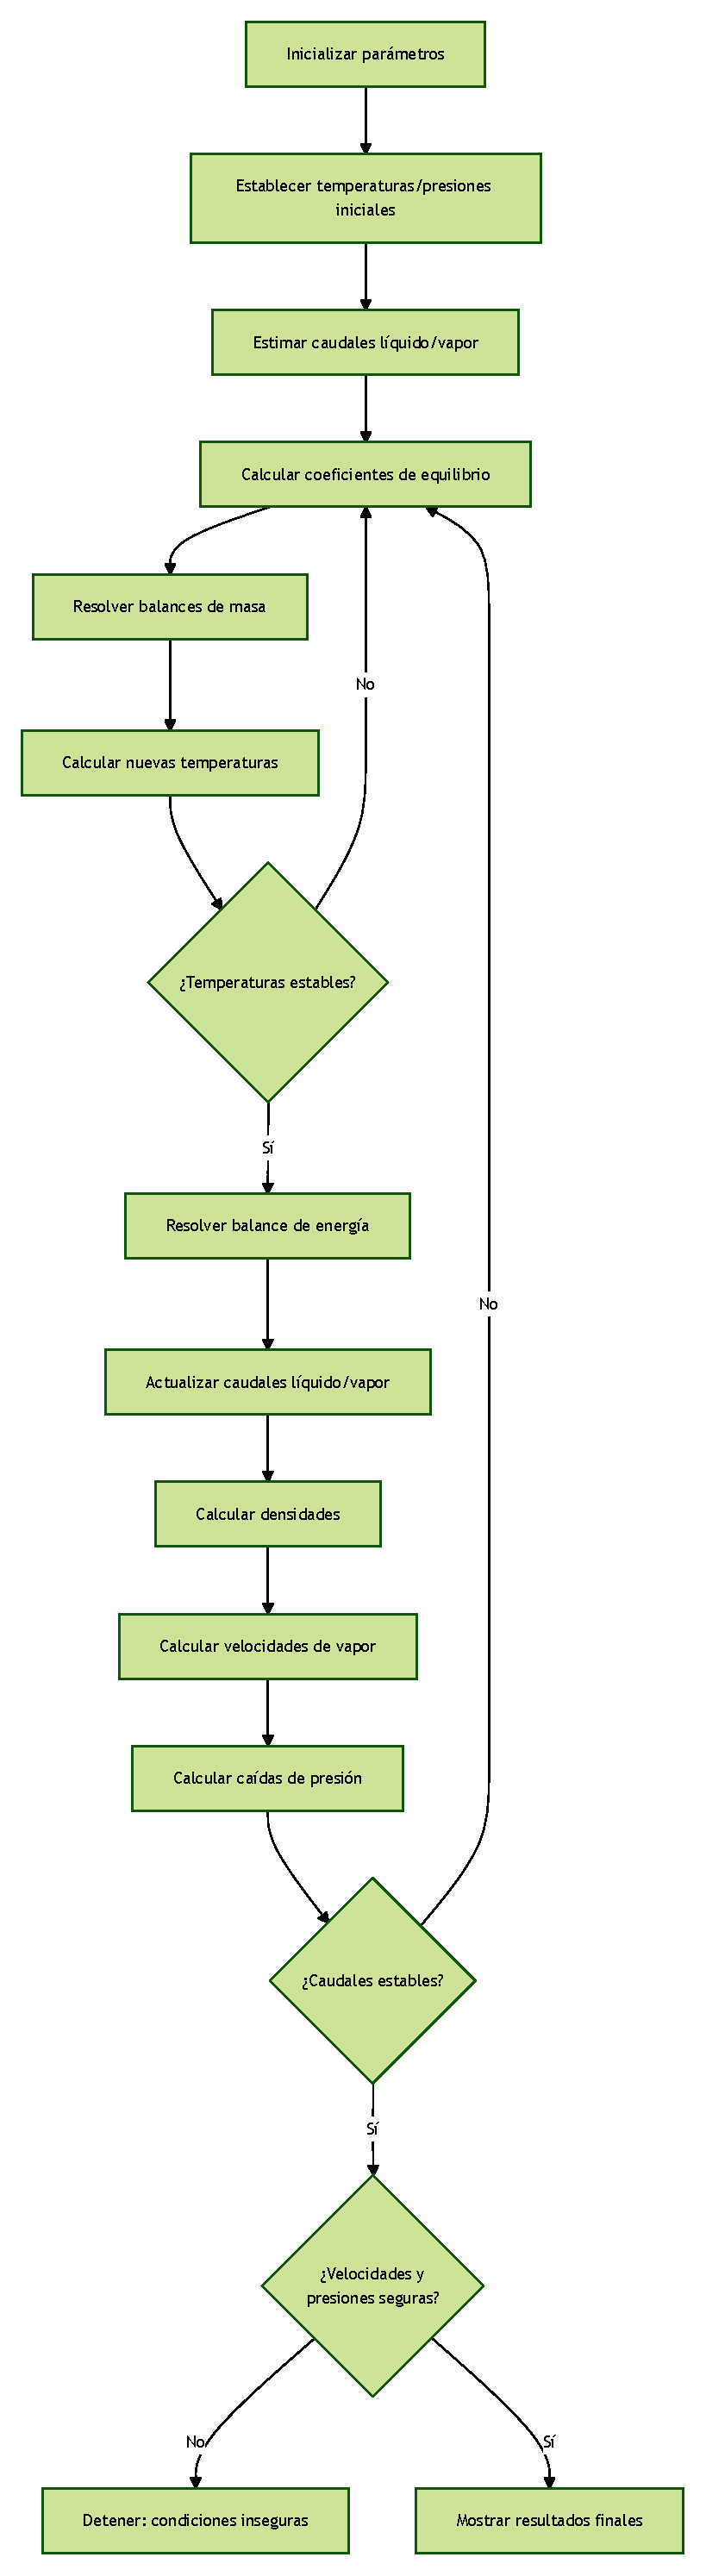
\includegraphics[height=0.85\textheight]{../resources/flowcharts/algoritmo_mesh.pdf}
      \caption{Algoritmo para la resolución del modélo matemático de la columna de destilación fraccionada.}
\end{figure}
